
\documentclass[11pt]{article}
\usepackage{graphics}
\usepackage{amsmath, amsthm, amssymb, latexsym}
\usepackage{hyperref}
%\usepackage[firstpage]{draftwatermark}
\usepackage{draftwatermark}
%\newtheorem{theorem}{Theorem}
%\newtheorem{definition}{Definition}
%\newtheorem{lemma}{Lemma}
%\newtheorem{corollary}{Corollary}

\begin{document}

\title{\textbf{Collecting Data with Unlock}}
\author{James Percent \\
  james@shift5.net}
\date{\today}
\parskip 11pt
\parindent 0pt


\maketitle

%\tableofcontents

\section{Overview}

This document provides details about using the Unlock framework, on the Mouth workstation, to collect data for offline analysis.  Section~\ref{unlock} covers Mouth account setup, Unlock software setup and MOBIlab hardware setup, and Section~\ref{collector} covers collecting data.

\section{Setup}\label{unlock}

A Mouth account is required to get started.  If you do not have a Mouth account, then send me an email and I'll create 1 for you.  

Next, login to Mouth and launch the Git Bash Shell.  To launch the Git Bash Shell, click Start Menu$\rightarrow$Git Bash Shell.  See Figure~\ref{fig:gitbash}.  

Note that the images in this document have high enough resolution to clearly read the text on them, so if you're having trouble reading the text, then use the Zoom In feature of your PDF viewer to increase the size of the image.

The next step is Github configuration.  Github needs to be configured with your public ssh key from Mouth.  You do not have a public key on Mouth by default, so we need to generate 1 using ssh-keygen.  After we generate a public key, we need to upload it to Github.  Finally, after the public key is uploaded, we can clone the repo.

Figure~\ref{fig:bash-cmds} shows the commands that need to be run from Mouth; in particular note that the generated public key is located in the .ssh directory of your home directory; also note, public keys end in $.pub$.  To upload the key to Github, click on the Account settings icon, and, after that page loads, click on SSH Keys link.

The MOBIlab device must be connected to collect data.  Connecting the MOBIlab to Mouth consists of 2 steps: powering on the MOBIlab and connecting its USB fob.  The MOBIlab USB is the 1 with the green key-ring identifier.

\begin{figure}[]
\resizebox{\textwidth}{!}{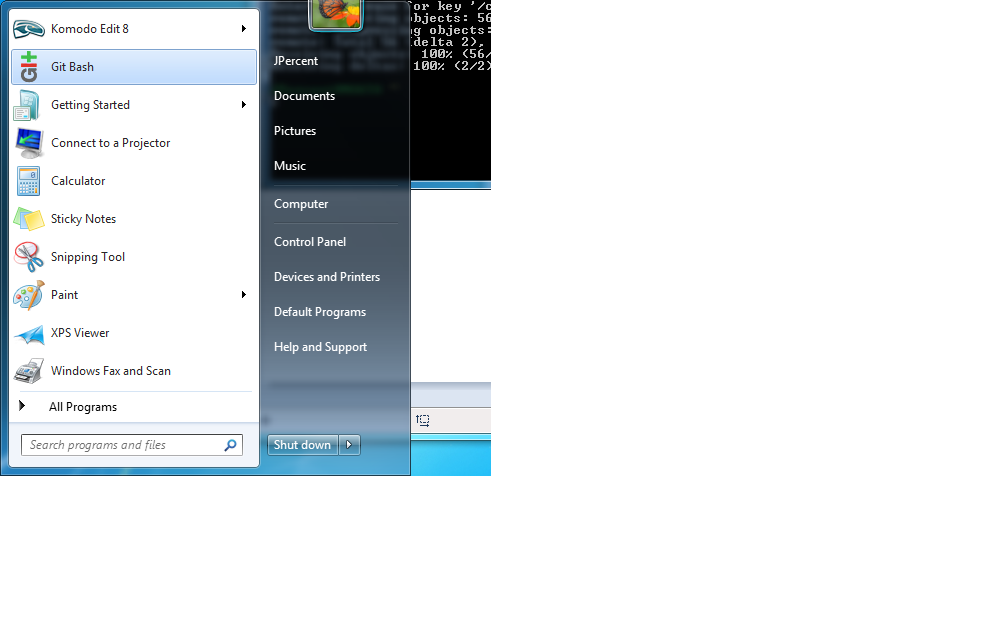
\includegraphics{images/git-bash0.png}}
\caption{\label{fig:gitbash} Git bash shell}
\end{figure}

\begin{figure}[]
\resizebox{\textwidth}{!}{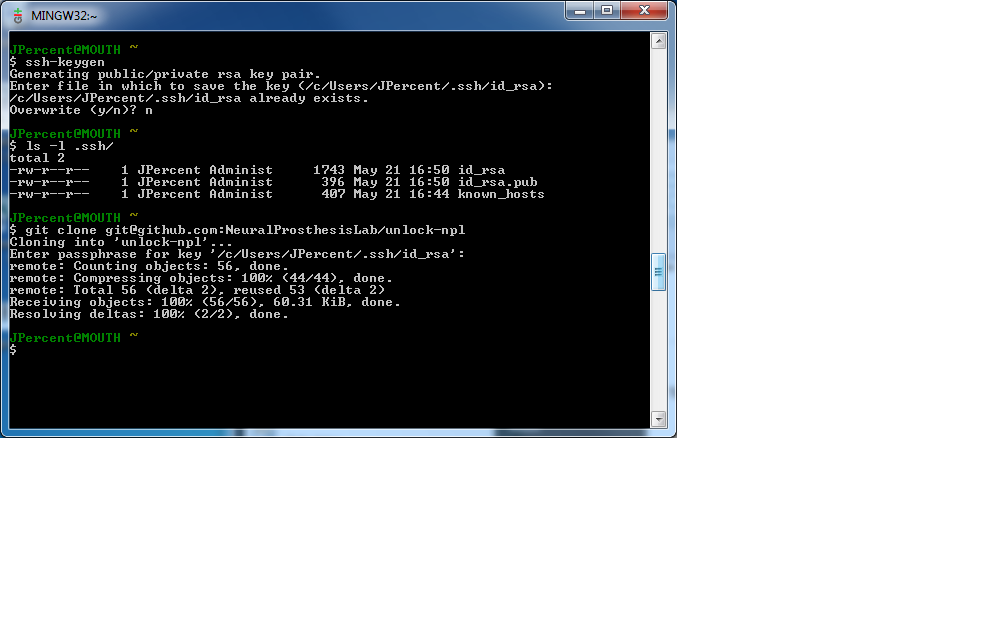
\includegraphics{images/bash-cmds.png}}
\caption{\label{fig:bash-cmds}  Bash commands }
\end{figure}

\section{Collecting Data}\label{collector}

After completing the steps in Section~\ref{unlock}, a directory called unlock-npl should exist in your home directory; enter this directory.  Collector.py is the program that we use to collect data.  Running the collector is simple.  To see the options run the following command.
\begin{verbatim}
	$ python collector.py --help
\end{verbatim}
Running an m-sequence visualization, with 4 cues, separated by 5 seconds, can be accomplished by executing the following command.  
\begin{verbatim}
	$ python collector.py -v left,right,up,down -m
\end{verbatim}
The output file consists of a sequence of samples separated line breaks.  Each sample consists of $n = channels + cue$ integers, separated by tabs.  For example, a 4 channel sample would look like the following.
\begin{verbatim}
11123	-2123	23456	1234	0
\end{verbatim}
The cue will be the last integer in the sequence.  A cue value can only be $0$ or $1$.  Figure~\ref{fig:cmds} shows the help output and some possible executions.  The default number of channels is 4, the default duration between cue events is 5 seconds, and the default output file will be named gtec concatenated with a timestamp.  Figure~\ref{fig:mseq} shows what an m-sequence visualization looks like.

\begin{figure}[]
\resizebox{\textwidth}{!}{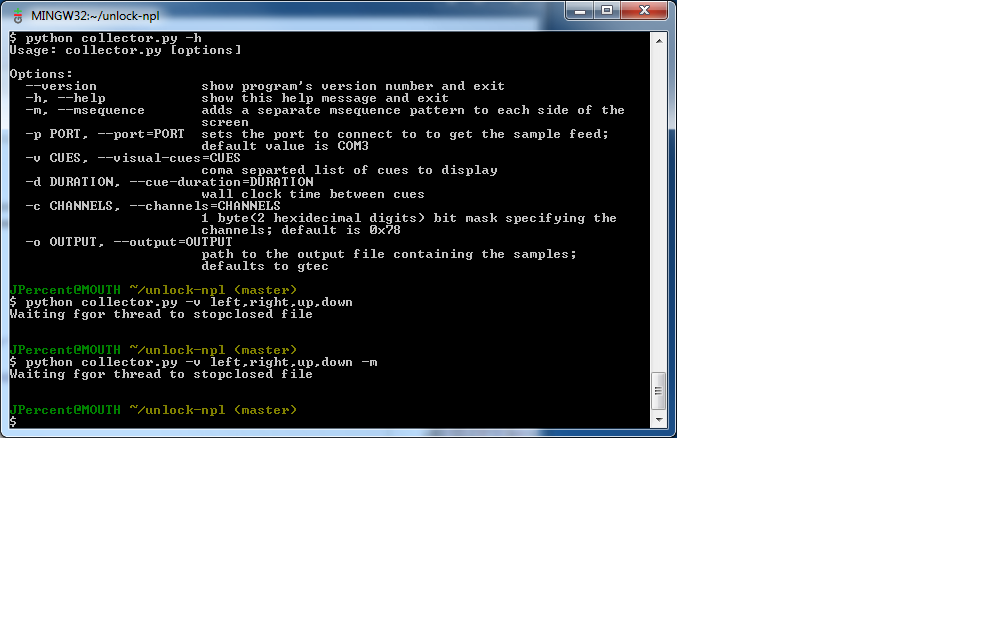
\includegraphics{images/commands.png}}
\caption{\label{fig:cmds}  Example collector usage}
\end{figure}

\begin{figure}[]
\resizebox{\textwidth}{!}{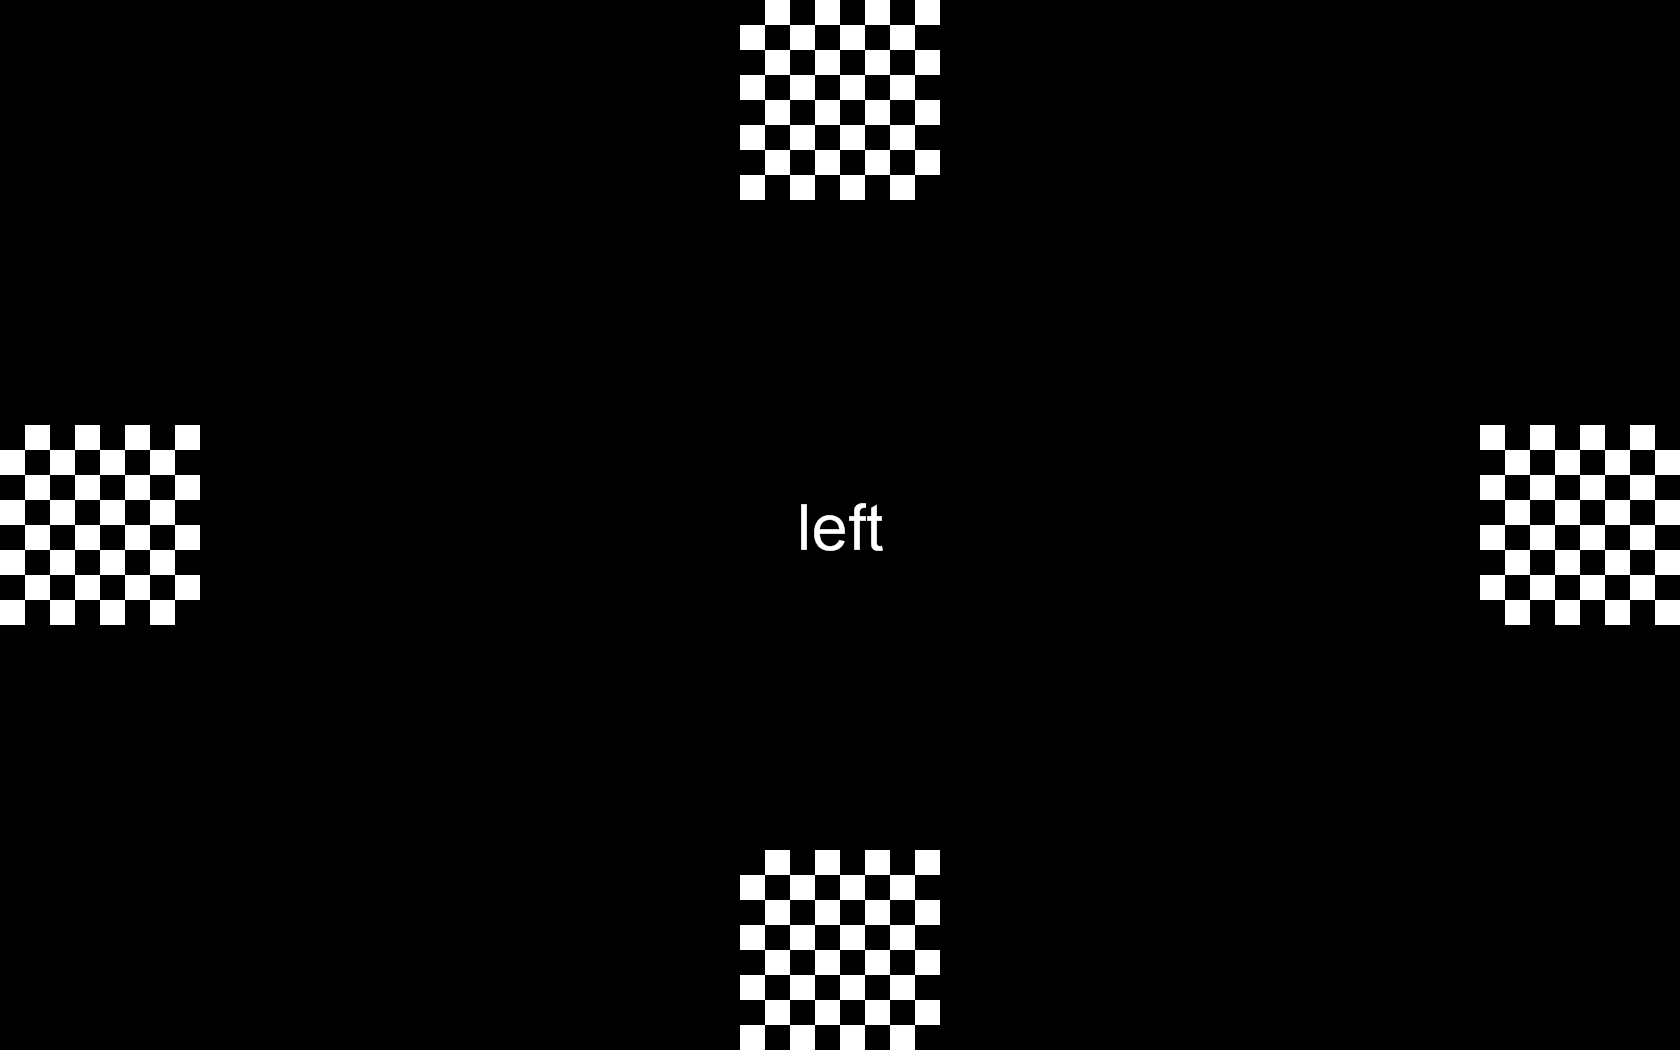
\includegraphics{images/msequence.png}}
\caption{\label{fig:mseq}  Example of running the m-sequence collector}
\end{figure}

%\begin{thebibliography}{99}
%\bibitem{unlock} http:\/\/github.com/NeuralProsthesisLab/unlock-npl.
%\bibitem{mobilab} http:\/\/www.gtec.at\/Products/Hardware-and-Accessories\/g.MOBIlab-Specs-Features
%\end{thebibliography}

\end{document}
